%!TEX root = ../../report.tex
\section{Mapping with Location noise}
\label{sec:mapping_with_location_noise}

Traditional approaches to occupancy grid mapping assumes ideal localization \cite{probRob}. 
Hence, the mapping amounts to updating the map with an inverse sensor model, like described in section \vref{sec:laser_range_sensor}.
This section investigates methods to improve mapping by incorporating localization noise.
While it is unrealistic to map the world exactly without knowing the exact pose of the robot, it is possible to adjust the sensor model based on the size of the estimated localization error.

\subsection{Simulation Setup}
The MiR-100 robot estimates its pose with an adaption of the ROS implementation \cite{ros_amcl} of the Adaptive Monte Carlo Localization(AMCL) \cite{Thrun200199}. AMCL uses a particle filter and a known map to track the robot's pose. 

The estimated uncertainty on the localization is described with a covariance matrix. 
The covariance matrices for some of the poses the robot visited during navigation at SCAN A/S is visualized as contour plots around the robots pose(green) in figure \vref{fig:amcl_covariance}. 
The figure shows that the estimated standard deviation on the positional error generally is around $10cm$. Around the corner the estimated standard deviation however increase to more than twice that. This is reasonably since the map used by AMCL for scan matching was wrong in the top left corner of figure \vref{fig:amcl_covariance}. The estimated angular error also doubles when the robot reaches the corner.

Figure \vref{fig:simulated_small_world} shows a map of the SCAN A/S production area which formed the basis for simulations. The corresponding map used by AMCL to estimate the robot pose is shown in \vref{fig:simulated_small_amcl_map}.
It is clearly visible from the maps that AMCL was missing information about the world. The lack of correspondence between the maps causes the covariance of the pose estimate to increase. 
Also shown is the true and estimated path the robot followed through the simulated environment. This simulation is used to compare the performance of the inverse sensor models described in this chapter. In order to ensure all methods was given the same input, data was logged while the robot followed the path shown in figure \vref{fig:test_map_setup}.

\begin{figure}[htbp]
	\centering
	\begin{subfigure}[t]{0.8\textwidth}
		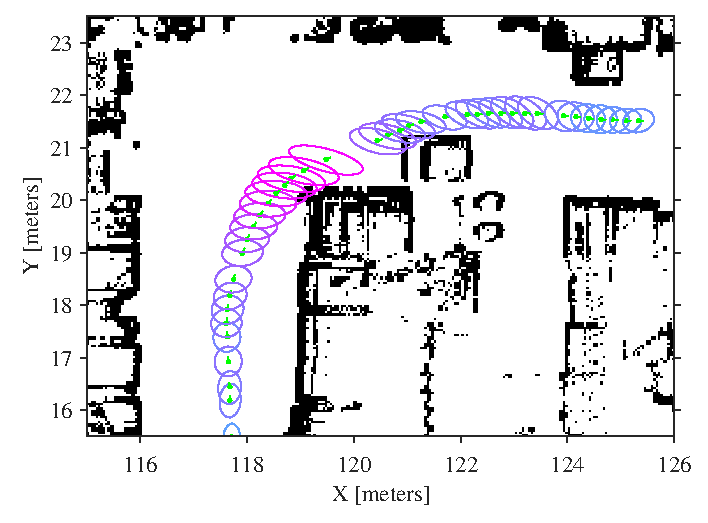
\includegraphics[scale=1.0]{figures/static_mapping/scan_region_with_poses}		
	\end{subfigure}
	\begin{subfigure}[t]{0.15\textwidth}
		\raisebox{1.15cm}{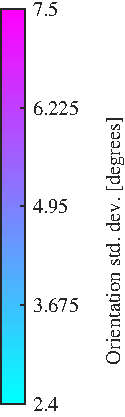
\includegraphics[scale=1.0]{chapters/evaluation/figures/localization_std_color_bar-crop}}
	\end{subfigure}
	\caption{Covariances estimated by AMCL in an industrial environment shown with contours marking one standard deviation around the robot's estimated pose(green).}
    \label{fig:amcl_covariance}
\end{figure}

\begin{figure}[htbp]
	\centering
	\begin{subfigure}[t]{0.4\textwidth}
		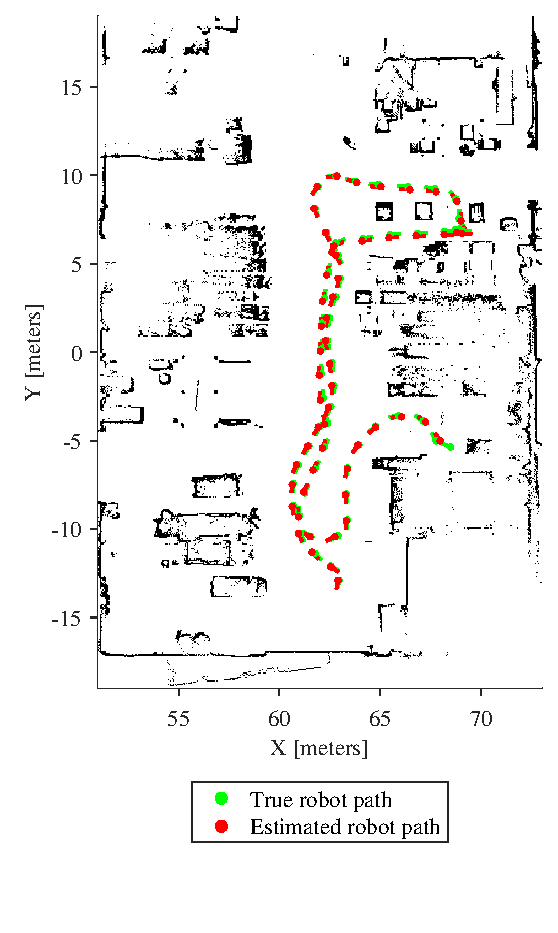
\includegraphics[width=\textwidth]{figures/static_mapping/simulation_poses_stage_map}
		\caption{World representation}
		\label{fig:simulated_small_world}
	\end{subfigure}
	\begin{subfigure}[t]{0.4\textwidth}
		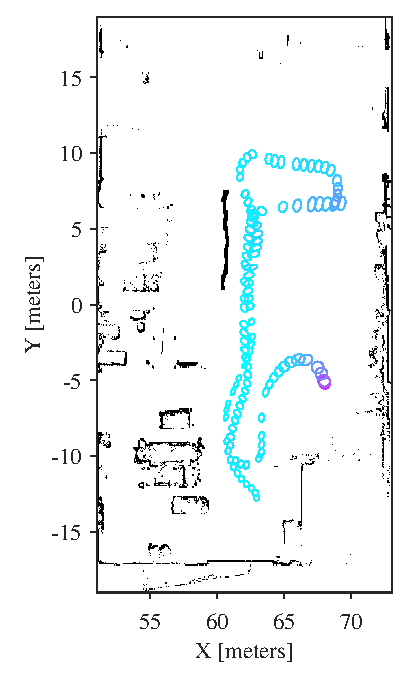
\includegraphics[width=\textwidth]{figures/static_mapping/simulation_poses_amcl_map}
		\caption{Map used by AMCL with estimation uncertainties shown around the estimated poses.}
		\label{fig:simulated_small_amcl_map}
	\end{subfigure}
   	\begin{subfigure}[t]{1\textwidth}
        \centering
        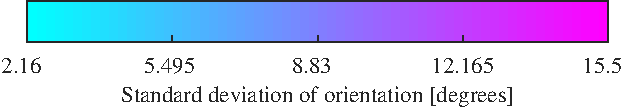
\includegraphics[scale=1.0]{figures/static_mapping/simulation_poses_amcl_map_bar-crop}
    \end{subfigure}
	\caption{Simulation of a MIR robot moving with imprecise location.}
	\label{fig:test_map_setup}
\end{figure}

\subsection{Reduced Ideal Inverse Sensor Model}
\label{sec:reduced_ideal_sensor_model}
The ideal inverse sensor model can be modified to avoid overconfidence in sensor measurements, by decreasing the update term in equation \ref{eq:occupancy_update} when the localization is wrong. 

\begin{figure}[htbp]
	\centering
	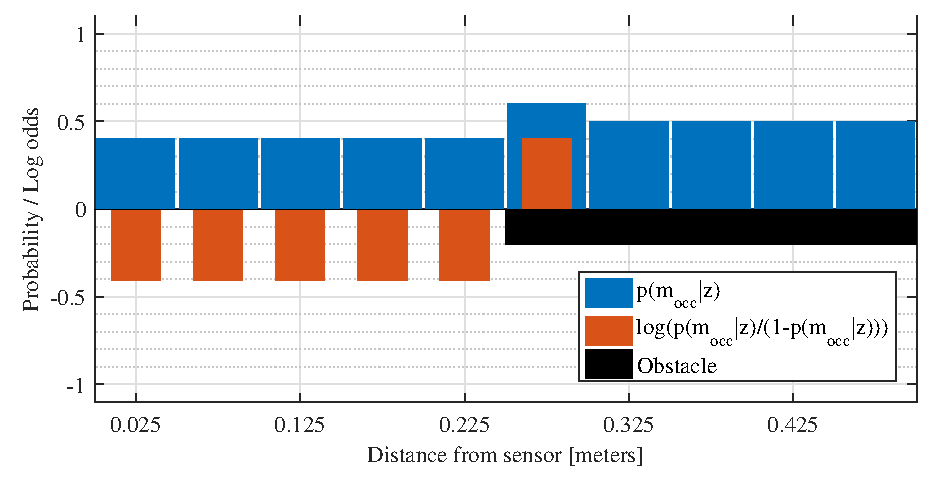
\includegraphics[scale=1]{figures/static_mapping/reduced_ideal_sensor_model}
	\caption{Reduced Ideal inverse sensor model}
	\label{fig:reduced_ideal_sensor_model}
\end{figure}

A reduced version of the ideal inverse sensor model is shown in figure \vref{fig:reduced_ideal_sensor_model} where the occupancy probability when observing free is $0.4$ and at the measured $0.6$ distance($l$). 
Despite the decrease in update values, the model can have a tendency to be overconfident in long measurements when the orientation is wrong.
This results in a removal of inserted obstacles when ray-traces wrongly go through them due to localization errors.
These effects are similar to the ones shown in figure \ref{fig:particle_hector_sensor-croped}.
This is diminished by multiplying the log-odds values with equation \vref{eq:angle-weight}.
Where \(\theta \) is the standard deviation of the orientation estimate and \(l\) is the measured distance.
\begin{equation}
\label{eq:angle-weight}
w_{angle} = 
\begin{cases}
1 - ( 2 \cdot \theta \cdot z ), & \text{if } 2 \cdot \theta \cdot l < 1\\
0, & \text{otherwise}
\end{cases}
\end{equation}

\begin{equation}
\label{eq:pose-weight}
w_{pose} = 
\begin{cases}
1 - ( 2 \cdot \theta \cdot z + 2 \cdot (\sigma_x + \sigma_y) ), & \text{if } 2 \cdot \theta \cdot z + 2 \cdot (\sigma_x + \sigma_y) < 1\\
0, & \text{otherwise}
\end{cases}
\end{equation}

The uncertainty of the position estimates are also incorporated in the weight shown in equation \vref{eq:pose-weight}.
Where \(\sigma_x\) is the standard deviation of the position estimate in the x-direction and \(\sigma_y\) is the equivalent in the y-direction.
Both of the weight functions are also to be tested with the Elfes model.

\subsection{Monte Carlo Integration Inverse Sensor Model}
\label{sec:monte_carlo_sensor Model}
The Monte Carlo integration inverse sensor model proposed by Joubert, Brink and Herbst \cite{Joubert2014},  uses the fact that particles used in Monte Carlo localization with their likelihood weights (importance factors) approximates the robots uncertainty. 
It works by ray-tracing the sensor measurements with a weighted inverse sensor model from the particles' poses instead of the estimated pose. 
Equation \vref{eq:monte_carlo_sensor_model} shows how a log-odds occupancy cell is updated with the right most term consisting of a weighted ($w_t^j$) sum of inverse sensor models for $K$ particles.

\begin{equation}
log \frac{p(m_i|z_{1:t})}{1-p(m_i|z_{1:t})} = log \frac{p(m_i|z_{1:t-1})}{1-p(m_i|z_{1:t-1})} + \sum_{j=1}^{K} w_t^j log \frac{ p(m_i | z_t) }{ 1 - p(m_i | z_t) }
\label{eq:monte_carlo_sensor_model}
\end{equation}

It can be computational expensive to ray-trace the often several hundred measurements every tenth of a second from each of the often several hundreds of particles.
To avoid this, only the $K$ highest weighted particles is be used. 
This has the effect that the total sum of update values is reduced to the total sum of the weights for the used particles times the sensor model.
Depending on the distribution of the particles, the amount of changes applied to the map per measurement varies.
Depending on processing capability and rate of measurements the number of used particles might be increased.

When using $30$ particles the map is updated with a sensor measurement on each of the two sensors as shown in figure \vref{eq:monte_carlo_sensor_model}.
The sensors' frames are shown around the robots base frame as green and red lines.
It is clear that it only updates the map weakly since the particles are far spread. 
The obstacles are updated at different positions since the particles are located at different positions. With the many particles this results in blurred lines which has the highest value in the center.

The model uses a reduced ideal inverse sensor model similar to the one described in section \vref{sec:reduced_ideal_sensor_model}, where the probability for occupancy at the obstacle is $0.85$. The probability for free is set to $0.45$. 
It is chosen to optimize the reduced ideal inverse sensor model this way, since it is better at adding obstacles as shown in figure \vref{fig:particle_principle}.

The reason to the methods tendency to remove obstacle is that small differences in orientation between the particles results in ray-traces going through the obstacles as shown in figure \vref{fig:particle_principle}. The weights for the used particles has been normalized to make the rays clearly visible. 
The figure shows how most of the ray-traced inverse sensor models results in similar looking maps along the rays. 
It can be seen how the model have built a map where there is a small probability for occupancy along the rays with similar distance but rotated around the robot's pose (red square). This results in a wrongful removal of obstacles.
Even with the optimized inverse sensor model, obstacle details shown in figure \ref{fig:test_map_setup} are lost. 

\begin{figure}[htbp]
	\centering
	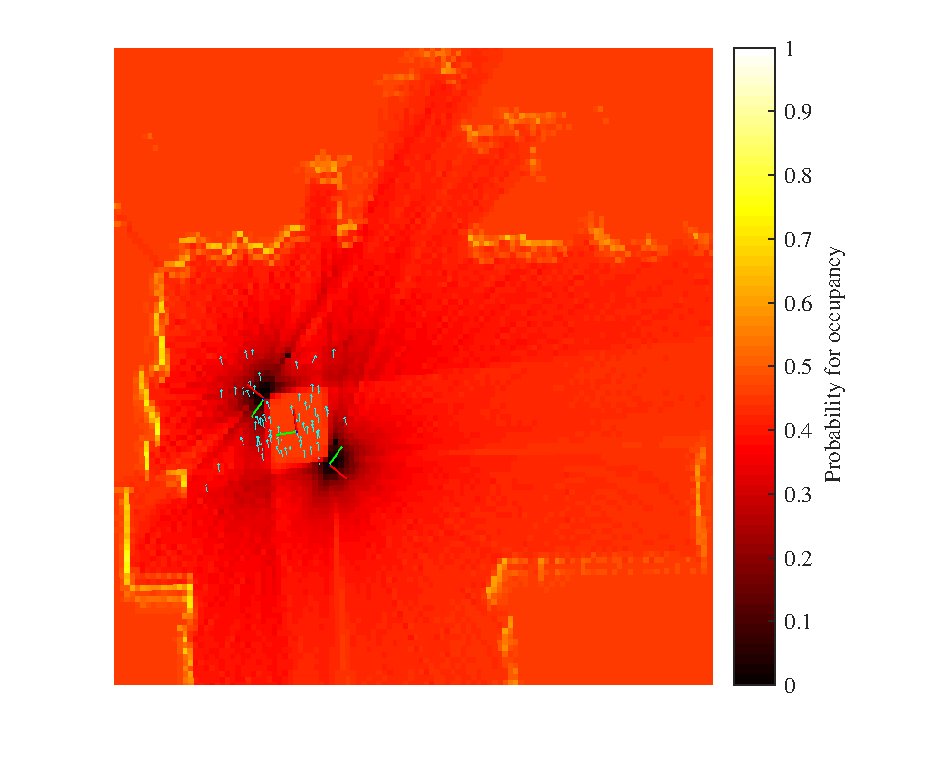
\includegraphics[scale=1.0]{figures/static_mapping/particle_principle}
	\caption{Map after ray-tracing with a modified reduced ideal inverse sensor model from all particles.}
	\label{fig:particle_principle}
\end{figure}

\begin{figure}[htbp]
	\centering
	\begin{subfigure}[t]{0.45\textwidth}
		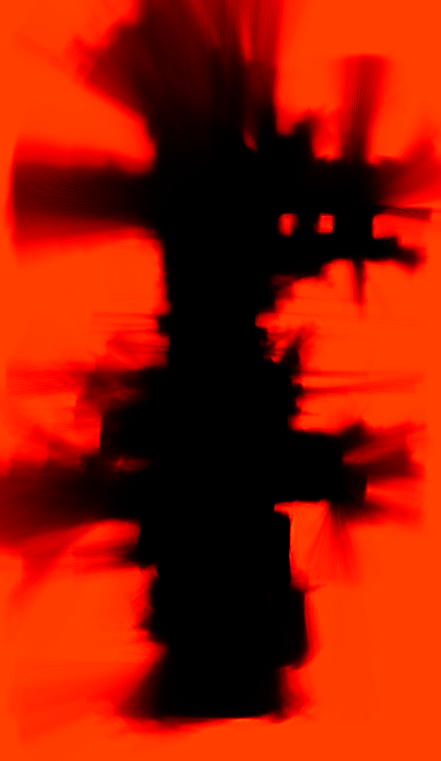
\includegraphics[width=\textwidth]{figures/static_mapping/monte_carlo_map_hector}
		\caption{Monte Carlo integration using Elfes inverse sensor model shown in figure \ref{fig:sensor_model_std_dev01}.}
        \label{fig:particle_hector_sensor-croped}
	\end{subfigure}
	\begin{subfigure}[t]{0.45\textwidth}
		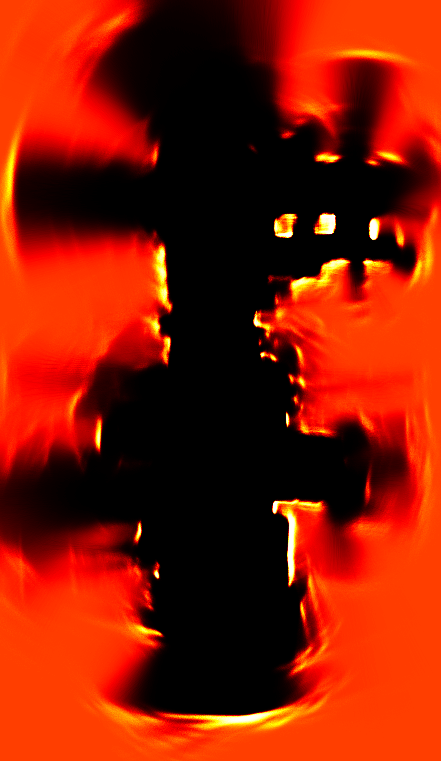
\includegraphics[width=\textwidth]{figures/static_mapping/monte_carlo_map_optimized}		
		\caption{Optimized inverse sensor model}
        \label{fig:particle_shot-croped}
	\end{subfigure}
	\caption{Mapping in simulation using Monte Carlo integration inverse sensor model with different sensor models for ray-traycing. The heatmap color scheme is used, see figure \vref{fig:particle_principle}}
\end{figure}

\begin{figure}[htbp]
    \centering
    \begin{subfigure}[t]{0.65\textwidth}
    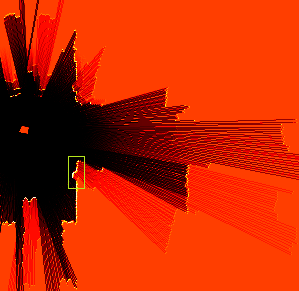
\includegraphics[height=3.5in]{figures/static_mapping/montecarlo_removing_obstacles}	
    \end{subfigure}
    \begin{subfigure}[t]{0.2\textwidth}
        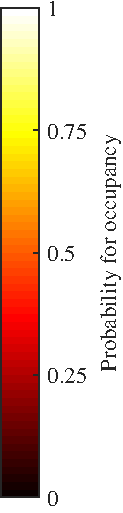
\includegraphics[scale=1.0]{figures/static_mapping/montecarlo_removing_obstacles_bar-crop}
    \end{subfigure}
    \caption{Example map with few LIDAR measurements mapped from the five highest weighted particles with Monte Carlo Integration. Within the green box obstacles are wrongly removed due to different orientation of particles.}
\end{figure}

\subsection{Cone Based Model}
An attempt to represent the pose uncertainty is an inverse sensor model similar to the model used for sonar sensors  \cite{probRob}.  
The idea is to represent the localization uncertainty in the model by representing it as shown in figure \vref{fig:cone_with_noise_top}.
For each laser range measurement the log-odds representation of the cone shown in figure is added to the OG map.
It shows the cone consisting of the center area, the left and right side cones. 
As the model is based on a sonar cone model, the values of a cell is determined by the distance \(l\) from the sensor's origin and the angle \(\theta\). 
The angle \(\theta\) is equal to the standard deviation of the orientation estimate. 
The width of the center area $l_2$ is determined by the sum of the position standard deviations $\sigma_x$ and $\sigma_y$ projected onto the line $b$. 

The value of a cell is determined by the distance from the line $b$. 
The value at the point $p$ in figure \vref{fig:cone_with_noise_top} is determined by the the distance \(l\).
The width $m$ of the marking cone is determined by the position standard deviations projected onto the line $l$.

It is possible to add a weight to each update value in the model. This weight is given by equation \vref{eq:cone-weight}.
\begin{equation}
\label{eq:cone-weight}
weigth = 
\begin{cases}
1 - ( 2 \cdot \theta \cdot l + l_2), & \text{if } 2 \cdot \theta \cdot l + l_2 < 1\\
0, & \text{otherwise}
\end{cases}
\end{equation}

\begin{figure}[htbp]
	\centering
	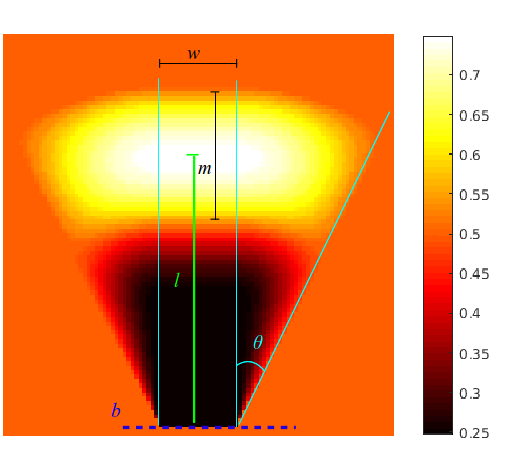
\includegraphics[width=\textwidth]{figures/static_mapping/cone_noise_top}
	\caption{Cone representing pose noise }
	\label{fig:cone_with_noise_top}
\end{figure}

\subsection{Comparison of Inverse Sensor Models}
In order to compare the various mapping methods a metric for determining the accuracy of a map is required. One of the methods for comparing two occupancy maps is the Map Score, first proposed in \cite{MoravecMartin}. The score is calculated as the squared error between the occupancy probability for each cell in two maps, as seen in equation \ref{eq:MapScore}.

\begin{equation}
\label{eq:MapScore}
\text{Map Score} = \sum_{i=1}^{N} (m_{i} - o_{i})^2
\end{equation}

$N$ is all cells in the ground truth map $m$ and the map to be scored $o$. 
This gives a simple result that indicates how different two maps are. As the score denotes the error between the two maps a lower score is preferable.  
However, as most maps contain vastly more free space than occupied space this might skew the result. 
Due to the majority of free space a map that assumes all cells are free can receive a  good score.
As the obstacles are vital parts of the map this characteristic is not desired. 
To overcome this we only use cells where the ground truth map $m$ is different from \(0.5\) and the tested map $o$ is above \(0.5\), this is denoted Sum of Squared Error (SSE).
As the SSE does not distinguish between the number of cells touched it is normalized with the number of cells in the tested map. This will be denoted the Mean Squared Error (MSE).  

\subsubsection{Results}
The methods was tested on the path through the simulated environment shown in figure \vref{fig:simulated_small_world}. 
The localization of the robot was not perfect due to differences between the world representation and the one used by AMCL.
As the world map has obstacle cells completely surrounded by other obstacle cells and therefore impossible for the robot to see the world map was adjusted before comparing with maps generated by different methods. Only obstacle cells with at least one neighboring free cell will be considered. Obstacle cells with no free cell neighbors are set to $0.5$. 

Figure \vref{fig:comparison_obstacle_error} shows the SSE for each method compared to the ground truth map in figure \vref{fig:simulated_small_world}. 
In this test the reduced ideal model with uncertainty decay received the lowest score. Both the Elfes and the reduced ideal model perform better when angle decay is used.
Similarly when position uncertainty is also used they score even better. 
 
Things change, however, when observing the results based on the MSE of figure \vref{fig:comparison_obstacle_error_per_cell}. 
Using the MSE the Monte Carlo method outperforms the other methods with a result of approximately \( 0.38\). The closes contestant the reduced ideal model with pose decay receive a score of approximately \(0.47\).

\begin{figure}[htbp]
	\centering
	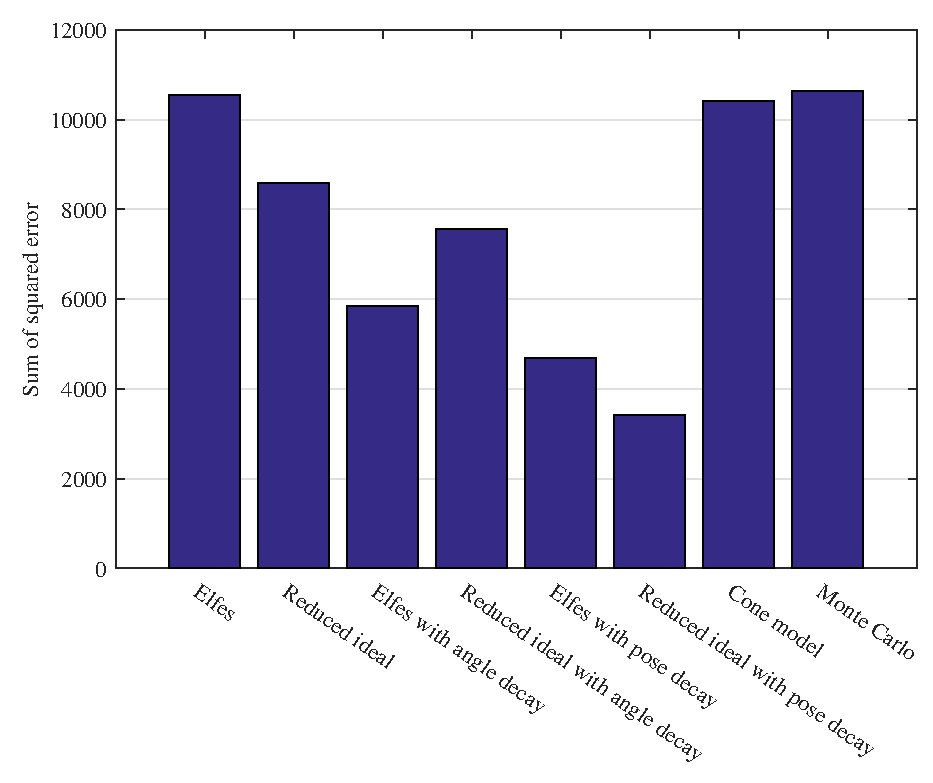
\includegraphics[scale=1]{figures/static_mapping/static_mapping_sse}
	\caption{SSE for differences between all estimated obstacle cells and all ground truth cells without a occupancy probability of $0.5$.}
	\label{fig:comparison_obstacle_error}
\end{figure}

\begin{figure}[htbp]
	\centering
	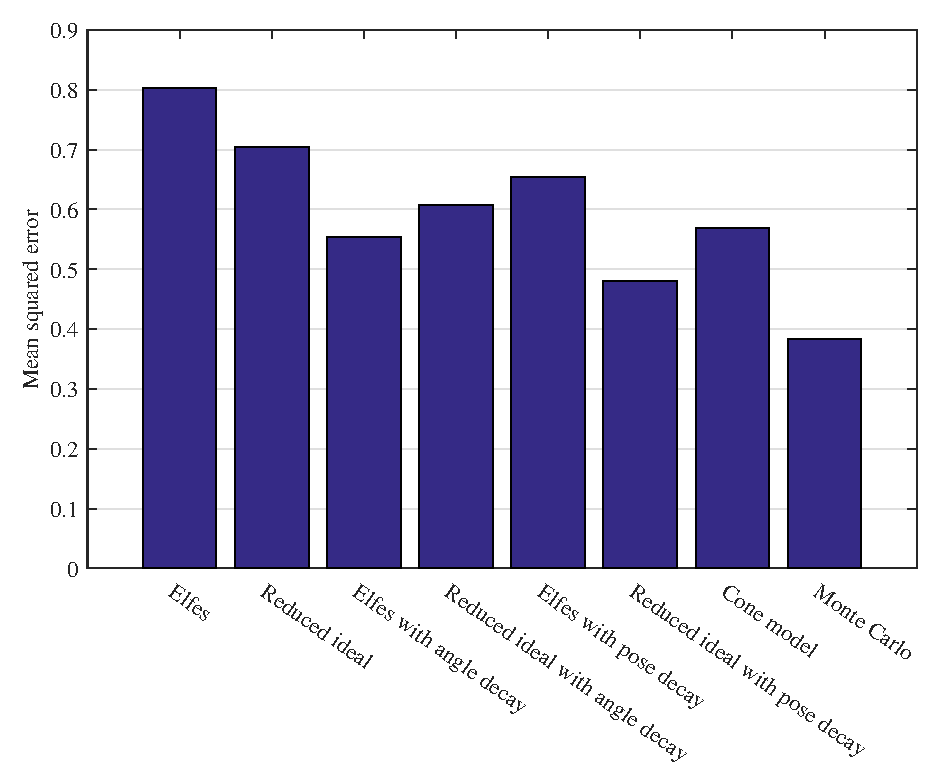
\includegraphics[scale=1]{figures/static_mapping/static_mapping_mse}
	\caption{Mean of the SSEs shown in figure \ref{fig:comparison_obstacle_error}.}
	\label{fig:comparison_obstacle_error_per_cell}
\end{figure}

The top scorers in both scoring systems are the Monte Carlo and the reduced ideal model with pose decay. As each of the two methods were at the top in one of the scoring methods, determining the best is not straight forward.

In order to further investigate the differences between the two methods the generated maps are compared and contrasted to the ground truth map. 
Figure \vref{fig:box_region_comparison} shows a comparison between the methods against the ground truth.
The Monte Carlo method produces larger occupied areas due to the way it incorporates the pose uncertainty. The occupied areas are blurred around the edges of the obstacles. 
This is in contrast to the reduced ideal model, which has marked sharper edges. 
These edges are however not perfectly located on the outer edge of the obstacles. 
This problem stems from the consistent pose error shown in figure \ref{fig:elfes_ideal_with_poses} that is not correctly handled by the pose decay. 

\begin{figure}[htbp]
	\centering
	\begin{subfigure}[t]{0.45\textwidth}
		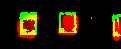
\includegraphics[scale=1.5]{figures/static_mapping/color_diff_monte_carlo}		
		\label{fig:monte_carlo_mapsec1}
		\caption{Monte Carlo method}
	\end{subfigure}
	~ %add desired spacing between images, e. g. ~, \quad, \qquad, \hfill etc. 
	%(or a blank line to force the subfigure onto a new line)
	\begin{subfigure}[t]{0.45\textwidth}
		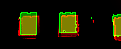
\includegraphics[scale=1.5]{figures/static_mapping/color_diff_ideal_decay}
		\label{fig:ideal_deacy_mapsec1}
		\caption{Reduced Ideal with decay}
	\end{subfigure}
	\caption{Region of the generated OG maps (red) and the ground truth (green). Following from that overlaps are to yellow.}
	\label{fig:box_region_comparison}
\end{figure}

For the further development of the mapping in dynamic environment it is chosen to use the reduced ideal model with pose decay. This method is considered most suitable for the task due to its ability to suppress pose uncertainties while still maintaining a fairly accurate representation of the environment. 
